\documentclass[12pt,fleqn,handout]{beamer}


\xdefinecolor{lavendar}{rgb}{0.8,0.6,1}
\xdefinecolor{olive}{cmyk}{0.64,0,0.95,0.4}
%\xdefinecolor{olive}{cmyk}{1,0,0,0}
\xdefinecolor{mag}{cmyk}{0.1,1,0,0.2}
\xdefinecolor{lblue}{rgb}{0,0,1.5}
\xdefinecolor{lred}{rgb}{1,0,0}
\xdefinecolor{mine}{cmyk}{1,0,0.2,0}
\xdefinecolor{bluel}{cmyk}{0.1,0,0.9,0.4}

\usepackage{amsmath,amssymb,dsfont,mathrsfs}
\usepackage{tikz,pgflibraryplotmarks}
\usepackage{multimedia}
\usepackage{wasysym}
\usepackage{rotating}
\usepackage{algorithm,algorithmic}
\usepackage{graphicx} % more modern
\usepackage{subfigure}
\usepackage{booktabs}

\usepackage{pgfplots}
\usepackage{verbatim}

\usepackage{setspace}
\newlength\iwidth
\newlength\iheight

\newcommand\makebeamertitle{\frame{\maketitle}}%
\graphicspath{{./images/}}
\setbeamertemplate{navigation symbols}{}
\addtobeamertemplate{navigation symbols}{}{%
    \usebeamerfont{footline}%
    \usebeamercolor[fg]{footline}%
	\insertshorttitle
    \;--
    \insertframenumber
}

\newcommand{\sectionstart}{
	\only<beamer>{
 	\begin{frame}% (fold)
 		\begin{centering}\Huge \insertsection \par\end{centering}
 	\end{frame}% frame the_application (end)
	}
 }


% make bibliography entries smaller
\usepackage{natbib}
\setbeamertemplate{bibliography item}{[\theenumiv]}
\renewcommand\bibfont{\scriptsize}
\setbeamertemplate{frametitle continuation}[from second]
\newcommand{\tcr}{\textcolor{red}}
\newcommand{\tcrd}{\textcolor{red}}
\newcommand{\tcb}{\textcolor{bluel}}
\newcommand{\tcm}{\textcolor{mag}}
\newcommand{\tcg}{\textcolor{olive}}

\newcommand{\R}{\mathbb{R}}
\newcommand{\C}{\mathbb{C}}

% bold lower-case for vectors
\newcommand{\bfa}{{\bf a}}
\newcommand{\bfb}{{\bf b}}
\newcommand{\bfc}{{\bf c}}
\newcommand{\bfs}{{\bf s}}
\newcommand{\bfm}{{\bf m}}
\newcommand{\bfd}{{\bf d}}
\newcommand{\bfe}{{\bf e}}
\newcommand{\bfu}{{\bf u}}
\newcommand{\bfy}{{\bf y}}
\newcommand{\bfx}{{\bf x}}
\newcommand{\bfh}{{\bf h}}
\newcommand{\bfw}{{\bf w}}
\newcommand{\bfv}{{\bf v}}
\newcommand{\bfr}{{\bf r}}
\newcommand{\bfz}{{\bf z}}
\newcommand{\bfp}{{\bf p}}


% bold upper-case for linear operators
\newcommand{\bfA}{{\bf A}}
\newcommand{\bfB}{{\bf B}}
\newcommand{\bfZ}{{\bf Z}}
\newcommand{\bfM}{{\bf M}}
\newcommand{\bfC}{{\bf C}}
\newcommand{\bfD}{{\bf D}}
\newcommand{\bfQ}{{\bf Q}}
\newcommand{\bfJ}{{\bf J}}
\newcommand{\bfG}{{\bf G}}
\newcommand{\bfI}{{\bf I}}
\newcommand{\bfP}{{\bf P}}
\newcommand{\bfK}{{\bf K}}
\newcommand{\bfY}{{\bf Y}}
\newcommand{\bfW}{{\bf W}}
\newcommand{\bfR}{{\bf R}}
\newcommand{\bfL}{{\bf L}}
\newcommand{\bfF}{{\bf F}}
\newcommand{\bfT}{{\bf T}}
\newcommand{\bfS}{{\bf S}}
\newcommand{\bfX}{{\bf X}}
\newcommand{\bfU}{{\bf U}}
\newcommand{\bfV}{{\bf V}}
\newcommand{\bfH}{{\bf H}}


\newcommand{\calF}{\mathcal{F}}



\newcommand{\hf}{{\frac 12}}
\newcommand{\bftheta}{{\boldsymbol \theta}}
\newcommand{\bfxi}{{\boldsymbol \xi}}

\newcommand{\bfLambda}{{\boldsymbol \Lambda}}
\newcommand{\bfSigma}{{\boldsymbol \Sigma}}
\newcommand{\bfepsilon}{{\boldsymbol \epsilon}}

\newcommand{\E}{\vec E}
\newcommand{\B}{\vec B}

\newcommand{\vu}{  {\vec {\bf u}}}

\newcommand{\grad}{  {\vec {\bf \nabla}}}

\newcommand{\lfrownie}{\textcolor{red}{\large{\frownie}}}
\newcommand{\lsmiley}{\textcolor{green}{\large{\smiley}}}

\newcommand{\curl}{\ensuremath{\nabla\times\,}}
\renewcommand{\div}{\nabla\cdot\,}
\newcommand{\divh}{\nabla_h\cdot\,}
\renewcommand{\grad}{\ensuremath{\nabla}}

\DeclareMathOperator*{\argmin}{arg\,min}


\title{ One-Layer Neural Networks}
\subtitle{Numerical Methods for Deep Learning}
\date{
}
\begin{document}

\makebeamertitle

\begin{frame}\frametitle{Motivation: Nonlinear Models}


In general, impossible to find a linear separator between classes
%$$ \bfC = \bfX \bfW + b $$

\begin{center}
	\begin{tabular}{cc}
		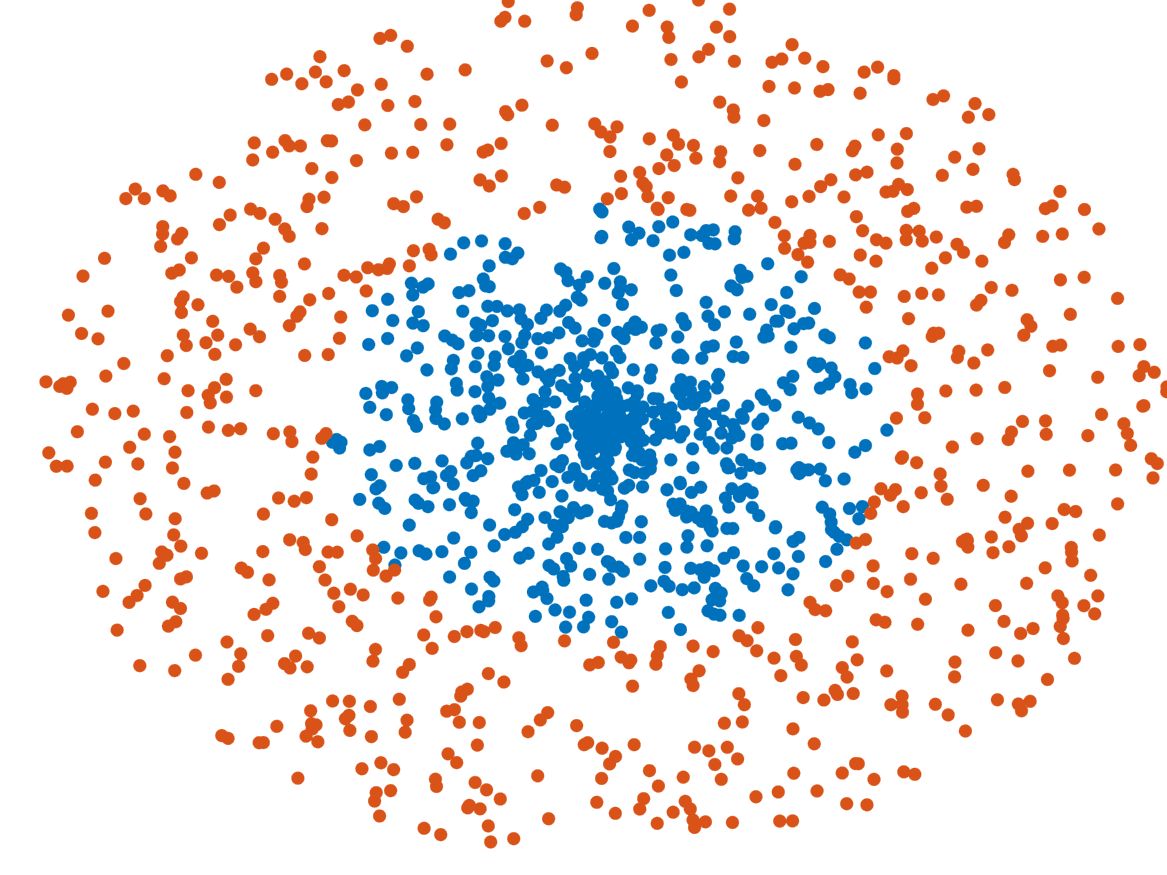
\includegraphics[width=45mm]{Circle-train} & 
		\invisible<beamer|1>{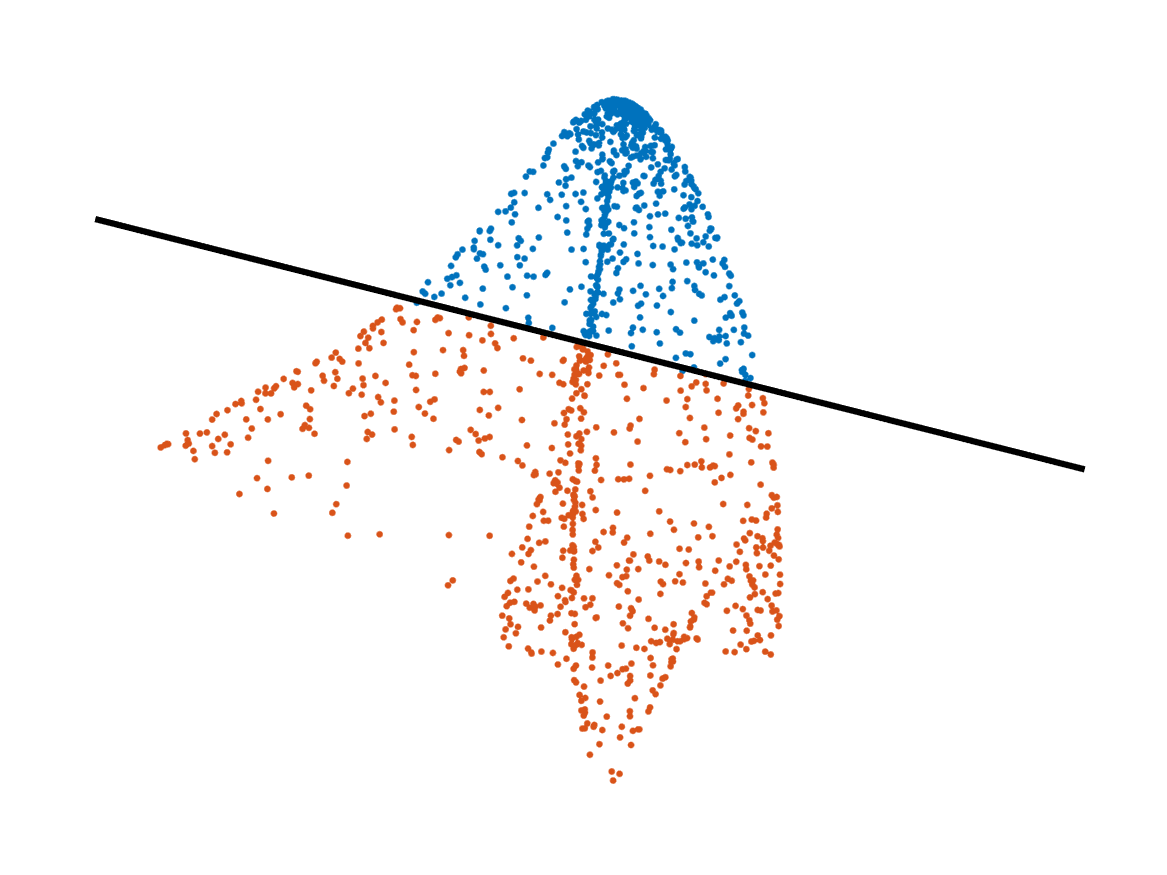
\includegraphics[width=45mm]{Circle-proptrain} }\\
		input features & \invisible<beamer|1>{transformed features}
	\end{tabular}
\end{center}

\bigskip

\invisible<beamer|1>{{\bf Goal/Trick}

Embed the points in higher dimension and/or move the points to make them
linearly separable}

\only<beamer|2>{}
\end{frame}

\begin{frame}[fragile]\frametitle{Learning the Weights}

Assume that the number of examples, $n$, is very large.

Using random weights, $\bfK$ might need to be very large to fit training data.

Solution may not generalize well to test data.

\bigskip
\pause

Idea: Learn $\bfK$ and $b$  from the data (in addition to $\bfW$)

$$ \min_{\bfK,\bfW,b} E(\bfW\sigma(\bfK \bfY + b), \bfC^{\rm obs}) + \lambda R(\bfW,\bfK,\bfb)$$

About this optimization problem:
\begin{itemize}
	\item more unknowns $\bfK \in \R^{m \times n_f}$, $\bfW \in \R^{n_c \times m}$, $b \in \R$
	\item  non-convex problem $\leadsto$ local minima, careful initialization
	\item need to compute derivatives w.r.t. $\bfK, b$
\end{itemize}


\end{frame}

\begin{frame}
	\frametitle{Non-Convexity}
	The optimization problem is non-convex. Simple illustration of cross-entropy along two random directions $d\bfK$ and $d\bfW$

	\begin{center}
		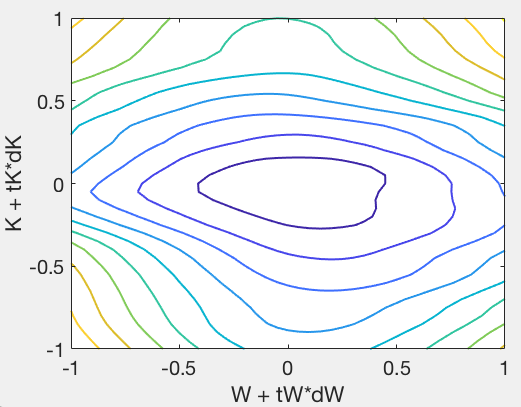
\includegraphics[width=.6\textwidth]{images/nonConvexitySingleLayer}
		
		(see \texttt{ESingleLayer\_PlotObjective.m})
	\bigskip
	
	Expect worse when number of layers grows!
	\end{center}

\end{frame}
\begin{frame}[fragile]\frametitle{Training the Neural Network}

\begin{itemize}
\item If non-convexity is not ``too bad'' can use standard gradient based methods
\item If non-convexity is ``ugly'' need to modify standard methods (stochastic kick)
\item If non-convexity is ``bad'' need global optimization techniques
\end{itemize}

	\begin{center}
	\begin{tabular}{ccc}
		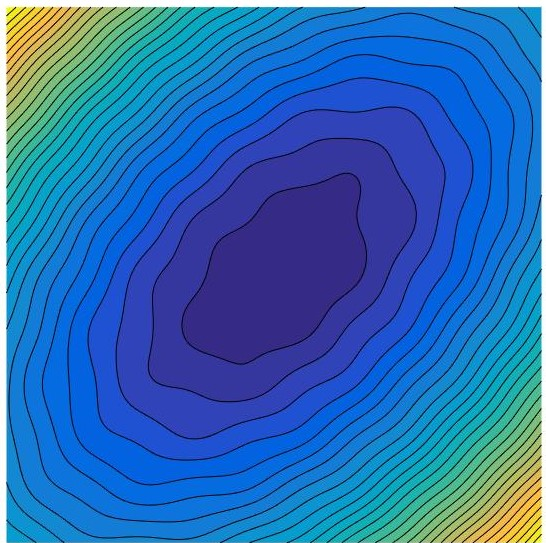
\includegraphics[width=.3\textwidth]{images/goodConv} &
		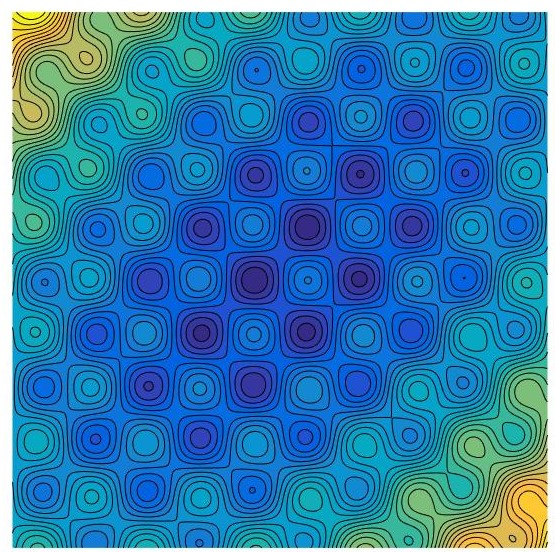
\includegraphics[width=.3\textwidth]{images/badConv} &
		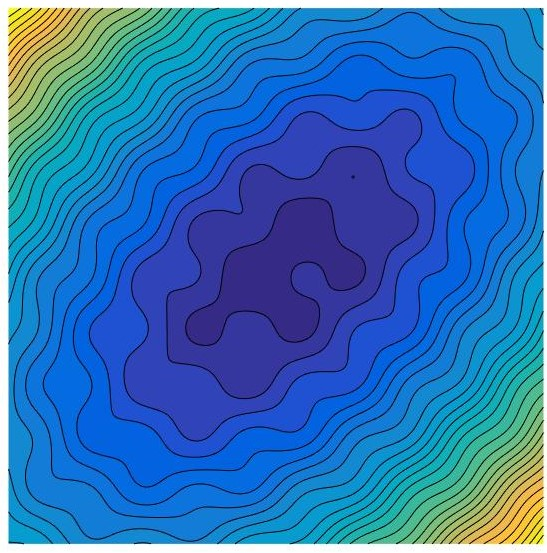
\includegraphics[width=.3\textwidth]{images/uglyConv} \\
		good & bad & ugly \\
		\end{tabular}
		\end{center}



\end{frame}
\begin{frame}[fragile]\frametitle{Recap: Differentiating Linear Algebra Expressions}

Easy ones:
\begin{align*}
 F_1(\bfx,\bfy) &= \bfx^{\top} \bfy  & \bfJ_{\bfx}F_1(\bfx,\bfy) = \bfy^\top\\
F_2(\bfA,\bfx)  &= \bfA \bfx         & \bfJ_{\bfx}F_2(\bfx,\bfy) = \bfA 
\end{align*}
\pause
How about
$$ F_3(\bfA,\bfX) =   \bfA  \bfX \quad \quad \bfJ_{{\rm vec}(\bfX)}F_3 = ??? $$
\pause
Recall that
$${\rm vec}(\bfA \bfX) = {\rm vec}(\bfA  \bfX \bfI) = (\bfI \otimes \bfA) {\rm vec} (\bfX) $$
Therefore:
$$ \bfJ_{{\rm vec}(\bfX)}F_3(\bfA,\bfX) = \bfI \otimes \bfA $$
\pause
\textcolor{red}{
Efficient mat-vec: } $\bfJ_{{\rm vec}(\bfX)}F \bfv = {\rm vec} ( { \bfA\ \rm mat}(\bfv) )$
	
\end{frame}


\begin{frame}[fragile]\frametitle{Training Single Layer Neural Network}

Assume no regularization (easy to add) and re-write optimization problem as 
\begin{eqnarray*}
 \min_{\bfW,\bfK,b}  E(\bfC^{\rm obs}, \bfZ,\bfW ) \quad \text{ with} \quad \bfZ = \sigma(\bfK\bfY + b)
\end{eqnarray*}

\bigskip
\pause

Agenda:
\begin{enumerate}
	\item compute derivative of ${\rm vec}(\bfZ)$ w.r.t. ${\rm vec}(\bfK), b$ 
	\item use chain rule to get
	\begin{align*}
		\bfJ_{{\rm vec}(\bfK)} E  & = \bfJ_{{\rm vec}(\bfZ)} E(\bfC^{\rm obs},\bfZ,\bfW) \ \bfJ_{{\rm vec}(\bfK)} \bfZ\\
		\bfJ_{b} E  & = \bfJ_{{\rm vec}(\bfZ)} E(\bfC^{\rm obs},\bfZ,\bfW) \ \bfJ_{b} \bfZ
	\end{align*}
	\item efficient code for mat-vecs with $\bfJ$ and $\bfJ^\top$
\end{enumerate} 
\end{frame}

\begin{frame}[fragile]\frametitle{Computing Jacobians}
$$
\bfZ = \sigma(\bfK\bfY + b)
$$
Recall that $\sigma$ is applied element-wise.
$$
	\bfJ_{{\rm vec}(\bfK)}\bfZ = {\rm diag}(\sigma'(\bfK \bfY + b)) (\bfY^\top \otimes \bfI)
$$
\pause
Efficient way to get matrix vector products
\begin{eqnarray*}
\bfJ_{{\rm vec}(\bfK)}\bfZ \bfv &=& {\rm diag}(\sigma'(\bfK \bfY + b)) (\bfY^\top \otimes \bfI)\bfv\\
                            &=& {\rm vec} \left(\sigma'(\bfK \bfY + b) \odot ( {\rm mat}(\bfv) \bfY )\right)
\end{eqnarray*}
And for transpose get
\begin{eqnarray*}
(\bfJ_{{\rm vec}(\bfK)}\bfZ)^\top \bfu &=& (\bfY \otimes \bfI) {\rm diag}(\sigma'(\bfK \bfY + b)) \bfu\\
                            &=& {\rm vec} \left(\sigma'(\bfK \bfY + b) \odot  {\rm mat}(\bfu)\bfY^\top\right) 
\end{eqnarray*}

\end{frame}




\begin{frame}[fragile]\frametitle{Class Problems: Derivatives of Single Layer}

\textbf{Derivations:}
\begin{enumerate}
	
	\item Compute $\bfJ_{b}\bfZ v$ and $(\bfJ_{b}\bfZ)^\top \bfu$

	\item Compute $\bfJ_{{\rm vec}(\bfY)}\bfZ  \bfv$ and $(\bfJ_{{\rm vec}(\bfY)}\bfZ)^\top  \bfu$
\end{enumerate}

\textbf{Coding:}
\begin{verbatim}
function[Z,JKt,Jbt,JYt,JK,Jb,JY] = singleLayer(K,b,Y)
% Returns Z = sigma(K*Y+b) and 
%                         functions for J'*U and J*V
\end{verbatim}

\textbf{Testing:}
\begin{enumerate}
	\item Derivative check for Jacobian mat-vec
	\item Adjoint tests for transpose, let $\bfv,\bfu$ be arbitray vectors
	$$
		\bfu^\top \bfJ \bfv \approx \bfv^\top \bfJ^\top \bfu
	$$
\end{enumerate}

\end{frame}


\begin{frame}[fragile]
	\frametitle{Putting Things Together}
	
	Implement loss function of single-layer NN
	$$
		E(\bfK,b,\bfW) \stackrel{def}{=} E(\bfC,\bfZ,\bfW), \quad \bfZ = \sigma(\bfK \bfY+b)
	$$
	
	
	\begin{verbatim}
		function [Ec,dE] = singleLayerNNObjFun(x,Y,C,m)
		% where x = [K(:); b; W(:)]
		% evaluates single layer and computes cross entropy 
		%        and gradient (extend for approx. Hessian)
	\end{verbatim}

	\bigskip
	
    Use
	\begin{enumerate}
		\item $\nabla_{\bfZ} E =  \bfW^\top \nabla_{\bfS} \ E(\bfS), \quad \bfS = \bfW\bfZ$
		\item $\nabla_{\bfK} E =  \bfJ_{\bfK}^\top \nabla_{\bfZ} E$
		\item $\nabla_{\bfb} E =  \bfJ_{\bfb}^\top \nabla_{\bfZ} E$
		\item $\nabla_{\bfW} E =  \nabla_{\bfS} \ E(\bfS) \bfY $
	\end{enumerate}
	
	
\end{frame}

\begin{frame}[fragile]
	\frametitle{Test Problem}
	
	Before going to real data, let us try the \emph{inverse crime}. Generate data
	\begin{verbatim}
		n  = 500; nf = 50; nc = 10; m  = 40;
		Wtrue = randn(nc,m);
		Ktrue = randn(m,nf);
		btrue = .1;

		Y     = randn(nf,n);
		Cobs  = exp(Wtrue*singleLayer(Ktrue,btrue,Y));
		Cobs  = Cobs./sum(Cobs,1);		
	\end{verbatim}
	
	\begin{center}
	Goal: Reconstruct \texttt{Wtrue, Ktrue, btrue}!  
	\end{center}
\end{frame}

\begin{frame}
	\frametitle{Gauss-Newton Method}
	
	\textbf{Goal:} Use curvature information to accelerate convergence
	$$
	\nabla_{\bfK} E(\bfK,b,\bfW) =  (\bfJ_\bfK \bfZ)^\top \nabla_\bfZ E(\bfW\sigma(\bfK \bfY+b),\bfC),
	$$
	where $\bfJ_\bfK \bfZ = \nabla_{\bfK} \sigma(\bfK \bfY+b)^\top$. This means that Hessian is
	\begin{equation*}
		\begin{split}
	\nabla_{\bfK}^2 E(\bfK) &  = (\bfJ_{\bfK}\bfZ)^\top  \nabla_\bfZ^2 E(\bfC,\bfZ,\bfW) \bfJ_{\bfK}\bfZ\\
	 & + \sum_{i=1}^{n}\sum_{j=1}^{m} \nabla_{\bfK}^2 \sigma(\bfK \bfY+b)_{ij} \nabla_\bfZ E(\bfC,\bfZ,\bfW)_{ij}
		\end{split}
	\end{equation*}
	
	First term is spsd and we can compute it.
	
	We neglect second term since
	\begin{itemize}
		\item can be indefinite and difficult to compute
		\item small if transformation is roughly linear or close to solution (easy to see for least-squares)
	\end{itemize}
	\begin{center}
		\textcolor{red}{do the same for $\bfb$ and use full Hessian for $\bfW$ $\leadsto$ ignore coupling!}
	\end{center}	
\end{frame}

\begin{frame}[fragile]
	\frametitle{Experiment: Adversarial Example}
	
	Suppose you have trained your network $\leadsto \bfK, b, \bfW$ so that validation loss is low. This means that for most examples $\bfy$, 
	$$
		\bfW \sigma(\bfK \bfy + b) \approx \bfc.
	$$
	
	An adversary might try to fool this classifier by adding a small perturbation $\bfd$ to the example to achieve a desired label $\hat{\bfc}$. 
	
	\bigskip
	
	Formulate as optimization problem
	$$
		\min_{\bfd} E(\bfW \sigma(\bfK (\bfy + \bfd) + b), \hat{\bfc})
	$$
	\begin{itemize}
		\item setup objective function
		\item think about constraints, regularization
	\end{itemize}
\end{frame}


\end{document}
\begin{frame}[fragile]\frametitle{Learning the weights}

{\bf Class problem}

\bigskip


Code a function
\small
\end{frame}


\end{document}
\begin{frame}[allowframebreaks]
	\frametitle{References}
\bibliographystyle{abbrv}
\bibliography{NumDNN}

\end{frame}



